\documentclass[runningheads]{llncs}
\usepackage[T1]{fontenc}
\usepackage{graphicx}
\usepackage{amsmath,amssymb}
\usepackage{booktabs}
\usepackage{xcolor}
\usepackage{tikz}
\usetikzlibrary{arrows.meta,positioning}
\usepackage[hidelinks]{hyperref}
\graphicspath{{figures/}}

% Result macros: every reported number lives in results_macros.tex, regenerated from the experiment
% output by scripts/fill_paper_results.py (outputs/experiment/results.json). \na marks a pending cell.
\newcommand{\na}{\textcolor{gray}{--}}
% Auto-generated by scripts/fill_paper_results.py. Do not edit by hand.
\providecommand{\na}{--}
\newcommand{\ablIouFull}{0.41}
\newcommand{\ablIouLm}{0.39}
\newcommand{\ablIouSeg}{0.30}
\newcommand{\ablIouTc}{0.42}
\newcommand{\ablLocFull}{27.1}
\newcommand{\ablLocLm}{28.6}
\newcommand{\ablLocSeg}{13.7}
\newcommand{\ablLocTc}{26.3}
\newcommand{\ablWFull}{0.115}
\newcommand{\ablWLm}{0.111}
\newcommand{\ablWSeg}{0.129}
\newcommand{\ablWTc}{0.106}
\newcommand{\diceCanon}{0.50}
\newcommand{\diceGroup}{0.66}
\newcommand{\fidCUT}{235.6}
\newcommand{\fidCUTCurvi}{72.3}
\newcommand{\fidCyc}{\textbf{192.2}}
\newcommand{\fidCycCurvi}{\textbf{67.9}}
\newcommand{\fidPhys}{315.3}
\newcommand{\fidPhysCurvi}{212.9}
\newcommand{\fidSCyc}{199.7}
\newcommand{\fidSCycCurvi}{104.2}
\newcommand{\fidSono}{294.7}
\newcommand{\fidSonoCurvi}{191.1}
\newcommand{\inReg}{0.065}
\newcommand{\iouCUT}{0.17}
\newcommand{\iouCyc}{0.11}
\newcommand{\iouPhys}{\textbf{1.00}}
\newcommand{\iouSCyc}{0.13}
\newcommand{\iouSono}{0.41}
\newcommand{\iouSonoCurvi}{0.54}
\newcommand{\kidCUT}{245.9}
\newcommand{\kidCUTCurvi}{55.9}
\newcommand{\kidCyc}{203.1}
\newcommand{\kidCycCurvi}{\textbf{55.6}}
\newcommand{\kidPhys}{294.3}
\newcommand{\kidPhysCurvi}{265.4}
\newcommand{\kidSCyc}{\textbf{196.9}}
\newcommand{\kidSCycCurvi}{84.2}
\newcommand{\kidSono}{306.5}
\newcommand{\kidSonoCurvi}{232.6}
\newcommand{\liverDice}{0.93}
\newcommand{\locCUT}{0.0}
\newcommand{\locCyc}{0.0}
\newcommand{\locPhys}{0.0}
\newcommand{\locSCyc}{0.0}
\newcommand{\locSono}{\textbf{26.3}}
\newcommand{\locSonoCurvi}{18.6}
\newcommand{\locality}{26}
\newcommand{\lungDice}{0.90}
\newcommand{\outReg}{0.005}
\newcommand{\softCanon}{0.35}
\newcommand{\softGroup}{0.75}
\newcommand{\tstrCUT}{0.031}
\newcommand{\tstrCyc}{0.032}
\newcommand{\tstrPhys}{0.049}
\newcommand{\tstrPhysCurvi}{0.097}
\newcommand{\tstrPhysCurviSd}{0.006}
\newcommand{\tstrPhysTent}{0.106}
\newcommand{\tstrPhysTentSd}{0.006}
\newcommand{\tstrSCyc}{0.026}
\newcommand{\tstrSono}{0.025}
\newcommand{\tstrSonoCurvi}{0.099}
\newcommand{\tstrSonoCurviSd}{0.011}
\newcommand{\tstrSonoTent}{0.124}
\newcommand{\tstrSonoTentSd}{0.007}
\newcommand{\ttaSeeds}{5}
\newcommand{\vesselDice}{0.72}
\newcommand{\wCUT}{0.246}
\newcommand{\wCyc}{0.266}
\newcommand{\wPhys}{0.064}
\newcommand{\wPhysCurvi}{0.056}
\newcommand{\wSCyc}{0.223}
\newcommand{\wSono}{\textbf{0.119}}
\newcommand{\wSonoCurvi}{0.115}

% Per-tissue in-the-loop results (organ-conditioned liver acquisition).
% Recognition = a REAL-trained organ recognizer J on held-out simulator content, crop-domain-matched
%   J, 3 seeds (scripts/premise/, aggregate.py). RL = organ-conditioned liver acquisition, 3 seeds,
%   held-out patients (scripts/train_organ_rl.py, agg_organ_rl.py). See docs/PREMISE_CHECK_RESULT.md.
\newcommand{\recSono}{0.48}
\newcommand{\recCut}{0.21}
\newcommand{\recCyc}{0.14}
\newcommand{\recPhys}{0.27}
\newcommand{\recCeil}{0.51}
\newcommand{\rlSono}{0.152}
\newcommand{\rlSonoSd}{0.004}
\newcommand{\rlCut}{0.144}
\newcommand{\rlCyc}{0.142}
\newcommand{\rlPhys}{0.142}
\newcommand{\rlStart}{0.11}
\newcommand{\rewSono}{0.32}
\newcommand{\rewPhys}{0.20}
\newcommand{\rewCut}{0.18}
\newcommand{\rewCyc}{0.16}
\newcommand{\rlSeeds}{3}


\begin{document}

\title{SonoSPADE: Real-Time, Per-Tissue Ultrasound Texture Synthesis for Closed-Loop Acquisition}
\titlerunning{Real-Time Per-Tissue Ultrasound Synthesis for Closed-Loop Acquisition}
\author{Thanapong Intharah\inst{1} \and Zhichao Gao\inst{2} \and Hao Dong\inst{2}}
\authorrunning{T. Intharah et al.}
\institute{Visual Intelligence Laboratory, Khon Kaen University, Khon Kaen, Thailand\\
\email{thanapong.intharah@gmail.com}
\and School of Computer Science, Peking University, Beijing, China}
\maketitle

\begin{abstract}
A closed-loop simulator for learning ultrasound \emph{acquisition} renders a new B-mode frame at every agent step, so its texture stage must be fast and controllable. 
Realism-first diffusion is far too slow to run in the loop, and global sim-to-real translators use a single appearance map across the whole image, giving no per-tissue control. 
We present \emph{SonoSPADE}, a per-tissue ultrasound texture stage that is real-time and GPU-free, trained unpaired with no real labels. 
The generator is conditioned on \emph{both} a physics render and the tissue label slice. 
A segmenter, pretrained for free on aligned simulator pairs and then frozen, pseudo-labels the real pool for an OASIS-style discriminator and drives a per-tissue consistency loss. 
A single pass runs at $15$ to $85$ frames per second \emph{without a GPU}, two to three orders of magnitude faster than diffusion. 
On the public Kaggle abdominal set, when we change a region's tissue label, only that region's texture changes, while methods that ignore the label do not react at all (label-swap locality ${\approx}\,26$, versus $0$). 
Per-organ intensity matches real about $2\times$ better than any learned baseline, and structure is preserved $2.4\times$ better; on whole-frame FID/KID it trails by design. 
As a first in-the-loop proof of concept, on an organ-conditioned task scored by a \emph{fixed} real-trained recognizer shared across texture stages, the per-tissue reward gives the highest ground-truth liver visibility in all three seeds. Code and the reproducible pipeline are released.
\keywords{Ultrasound synthesis \and Semantic image synthesis \and Real-time synthesis \and Closed-loop simulation \and Sim-to-real.}
\end{abstract}

\section{Introduction}
We study how to learn ultrasound \emph{acquisition} in simulation: an agent moves a virtual probe and observes the B-mode frame it would produce, so a texture stage must render a new frame at every step. 
The stage must be fast, must run on an ordinary computer, and must be controllable, so that the agent's actions map to anatomy. 
Realism-first synthesizers do not meet these needs. Diffusion produces high-quality ultrasound but takes seconds per frame~\cite{stojanovski2023echofromnoise}, far too slow for a loop that uses millions of frames. 
Global sim-to-real translators work on the grayscale image alone~\cite{song2024scyclegan}, applying one appearance map to the whole frame, so they cannot make sure that liver reads as liver and kidney as kidney. 
Yet the pipeline already knows the anatomy: a canonical label slice drives a physics B-mode with acoustic shadowing, a depth-varying point spread function, and correlated speckle. We make the learned stage \emph{per tissue} by conditioning it on that label slice, and keep it single-pass so it runs in real time without a GPU. 
This improves on both semantic image synthesis~\cite{park2019spade} and segmentation-consistent CT-to-US translation~\cite{song2024scyclegan}; realism-first anatomy-consistent synthesizers~\cite{vitale2025realism} aim at offline augmentation at higher fidelity, while we trade fidelity for the speed and per-tissue control a texture stage needs in the loop.

Two design choices set SonoSPADE apart. First, the generator is conditioned on \emph{both} the physics render and the label, so it refines a tissue-correct render instead of inventing ultrasound from CT.
Second, a frozen segmenter, pretrained for free on aligned pairs, supplies both the OASIS-style discriminator's pseudo-labels~\cite{sushko2021oasis} and a per-tissue consistency term, removing SPADE's need for paired real data~\cite{park2019spade}. 
A one-sided contrastive backbone~\cite{park2020cut} keeps training on a laptop without CUDA. 
Our contributions are:
\begin{itemize}
\item A real-time, GPU-free per-tissue texture stage: a single pass at $15$--$85$ frames/s on a laptop with no discrete GPU, two to three orders of magnitude faster than diffusion, that runs in the loop without becoming the bottleneck.
\item A physics-conditioned dual-input generator, conditioned on \emph{both} the physics render and the label slice, giving per-tissue control (relabel a region and only its texture changes) with free unpaired segmentation consistency, so no real labels are needed.
\item A per-tissue evaluation (per-class Wasserstein, a label-swap locality metric, speckle SNR/GLCM), plus a diagnosis and two fixes (a sector remap and test-time adaptation) that move SonoSPADE from worst to ahead of the raw render on downstream transfer.
\item A first in-the-loop proof of concept: under a \emph{fixed} real-trained recognizer shared across texture stages, the per-tissue reward gives the highest ground-truth liver visibility in all three seeds.
\end{itemize}

\section{Related Work}
\noindent\textbf{Semantic synthesis and label-consistent US.} SPADE conditions generation on a label map
via spatially-adaptive normalization~\cite{park2019spade}, and OASIS recasts the critic as a per-pixel
segmentation discriminator~\cite{sushko2021oasis}; both are supervised and label-only. We borrow the
adaptive conditioning but drive it from a physics render and supervise the discriminator with \emph{free}
pseudo-labels. A parallel line generates label-consistent US from anatomical models to train segmenters
(e.g.,\ a CycleGAN at $87$--$91$ Dice on cardiac structures~\cite{gilbert2021synthetic}); these
whole-image translators offer no per-tissue control, which we expose by conditioning on the label.
\noindent\textbf{Anatomy-consistent US synthesis.} Closest to us, Vitale et al.~\cite{vitale2025realism}
combine a segmentation-guided loss and polar (sector) training to suppress hallucinations and improve
realism; related structure-preserving translators include
S-CycleGAN~\cite{song2024scyclegan,zhu2017cyclegan} and CACTUSS~\cite{velikova2022cactuss}. These optimize
offline realism; we optimize per-frame latency for in-the-loop use, and add per-tissue \emph{conditioning}
(not merely a loss), a label-swap locality metric, and single-pass GPU-free inference. Semantic
diffusion~\cite{stojanovski2023echofromnoise} reaches higher fidelity but needs tens to hundreds of passes
per frame, too slow for an agent that uses millions of frames.

\section{Method}
Fig.~\ref{fig:pipeline} summarizes SonoSPADE. Let $x$ be a physics B-mode render and $\ell$ its one-hot
canonical tissue label slice ($K{=}13$ classes). The generator $G(x,\ell)$ refines $x$ into a realistic
frame; it is trained unpaired against a real pool $\mathcal{R}$ with three forces.

\begin{figure}[t]
\centering
\resizebox{0.63\linewidth}{!}{%
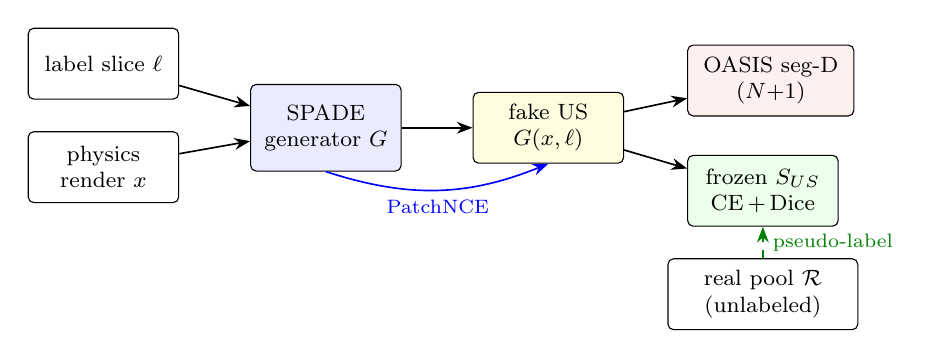
\begin{tikzpicture}[font=\footnotesize,
  box/.style={draw,rounded corners=2pt,align=center,inner sep=3pt,minimum height=9mm,text width=17mm},
  gen/.style={draw,fill=blue!8,rounded corners=2pt,align=center,inner sep=3pt,minimum height=11mm,text width=17mm},
  crit/.style={draw,fill=red!6,rounded corners=2pt,align=center,inner sep=3pt,minimum height=9mm,text width=19mm},
  arr/.style={-{Stealth[length=2mm]},line width=0.6pt}]
  \node[box] (label) {label slice $\ell$};
  \node[box,below=4mm of label] (phys) {physics render $x$};
  \node[gen,right=9mm of phys,yshift=5mm] (g) {SPADE\\generator $G$};
  \node[box,fill=yellow!12,right=9mm of g] (fake) {fake US\\$G(x,\ell)$};
  \node[crit,right=8mm of fake,yshift=6mm] (d) {OASIS seg-D\\$(N{+}1)$};
  \node[box,fill=green!8,right=8mm of fake,yshift=-8mm] (s) {frozen $S_{US}$\\CE\,+\,Dice};
  \draw[arr] (label) -- (g); \draw[arr] (phys) -- (g); \draw[arr] (g) -- (fake);
  \draw[arr] (fake) -- (d); \draw[arr] (fake) -- (s);
  \draw[arr,blue] (g.south) to[bend right=20] node[below,font=\scriptsize]{PatchNCE} (fake.south);
  \node[box,below=4mm of s,text width=22mm] (real) {real pool $\mathcal{R}$ (unlabeled)};
  \draw[arr,green!50!black,dashed] (real) -- (s.south) node[midway,right,font=\scriptsize]{pseudo-label};
\end{tikzpicture}}
\caption{SonoSPADE. The label slice and the physics render both condition the generator. A frozen
segmenter $S_{US}$, pretrained free on aligned simulator pairs, pseudo-labels the real pool for an OASIS
$(N{+}1)$ discriminator and enforces a per-tissue consistency loss; PatchNCE preserves content. No inverse
generator, no cycle loss.}
\label{fig:pipeline}
\end{figure}

\subsection{Physics-conditioned dual-input generator}
$G$ is a ResNet encoder-decoder whose residual and upsampling blocks are SPADE-normalized: a
parameter-free instance norm whose per-pixel scale and bias are predicted from the resized label map
$\ell$, so the semantic layout modulates activations at every scale~\cite{park2019spade}. The physics
render $x$ is the content stream, so $G$ refines a tissue-correct render instead of hallucinating anatomy.
Content is preserved by multilayer PatchNCE on $G$'s own encoder features~\cite{park2020cut} between $x$
and $G(x,\ell)$; there is no inverse generator and no cycle loss.

\subsection{Free unpaired segmentation consistency}
The simulator emits perfectly aligned $(x,\ell)$ pairs, so a compact U-Net~\cite{ronneberger2015unet}
segmenter $S_{US}$ is pretrained at no annotation cost, then \emph{frozen} and used two ways. (i)~It
pseudo-labels the unlabeled real pool, giving an OASIS-style $(N{+}1)$-class per-pixel discriminator $D$ a
semantic target for free~\cite{sushko2021oasis}: $G$ wins only when each synthesized pixel reads as its
conditioned tissue. (ii)~A consistency loss $\mathcal{L}_{seg}=\mathrm{CE}+\mathrm{Dice}$ requires
$S_{US}(G(x,\ell))$ to match $\ell$, so $G$ cannot collapse to a global recolor. The full objective is
\begin{equation}
\mathcal{L}=\mathcal{L}_{adv}^{\text{OASIS}}+\lambda_{nce}\mathcal{L}_{nce}
+\lambda_{seg}\mathcal{L}_{seg}+\lambda_{tc}\mathcal{L}_{tc},
\end{equation}
where $\mathcal{L}_{adv}$ uses class-balanced per-pixel cross-entropy, so rare tissues are not ignored.

\subsection{Grouped scheme and training}
Fat, GI wall, pancreas, muscle, and generic soft tissue have near-equal backscatter and render almost
identically, so $S_{US}$ and $D$ use a \emph{grouped} scheme (these five merge; distinct structures keep
their class) while $G$ still conditions on the full $K$ classes. Three light stabilizers help: a
temporal-consistency term $\mathcal{L}_{tc}$ requiring $G$ to commute with a small in-plane shift, an
OASIS-style LabelMix on $D$~\cite{yun2019cutmix}, and an R1 gradient penalty~\cite{mescheder2018r1}. The
deployed generator is an EMA of the training weights.

\section{Experiments}
\subsection{Setup}
We build on an ultrasound substrate that runs on an ordinary laptop: it renders a physics B-mode from a CT-derived canonical label volume (13 tissues via TotalSegmentator~\cite{wasserthal2023totalseg}) and exposes a label-conditioned translator interface. Free aligned $(x,\ell)$ pairs come from eight abdominal
CT cases with pose sweeps and domain randomization. 
For the real head-to-head, we use the public Kaggle abdominal ultrasound set~\cite{vitale2020realism}: every translator is trained on its $404$-frame real train split and evaluated on the disjoint $60$ annotated real frames (liver, kidney, gallbladder, spleen, vessels), a leakage-free real test on the same held-out content. 
Everything runs on Apple Silicon (MPS, no
CUDA).

\subsection{The label conditioning is genuinely per-tissue}
\label{sec:pertissue}
The central claim is that texture is per-tissue, not a global recolor. Holding the physics render fixed,
we relabel a tissue region and measure the texture change inside versus outside. A global recolor scores
near zero inside. SonoSPADE changes the region's own texture by $\inReg$ inside versus $\outReg$ outside,
a \emph{pooled} inside-to-outside ratio of about $13$. The label-swap locality metric in
Table~\ref{tab:main} is a stricter per-class summary: it averages each tissue's own inside/outside ratio,
giving $\locSono$ for SonoSPADE versus $0$ for every label-free translator by construction (supplementary
Fig.~S1). The per-class mean exceeds the pooled $13$ because tissues with very little out-of-region change
give large ratios. Per-class speckle SNR also shifts per tissue, confirming statistics learned per tissue,
not one uniform map.

\subsection{Free segmentation supervision}
Pretrained on the aligned pairs, $S_{US}$ reaches \liverDice{}/\lungDice{}/\vesselDice{} Dice on
liver/lung/vessels (acoustically distinct) on held-out patients. The canonical 13-class macro Dice is
capped at \diceCanon{} by indistinct soft tissues; merging them in the grouped scheme lifts it to
\diceGroup{} (merged soft-tissue class \softGroup{} versus \softCanon{}), with no change to distinct
tissues. This reflects B-mode acoustics, not a tuning trick.

\subsection{Comparison to baselines}
\label{sec:baselines}
Table~\ref{tab:main} compares raw physics, CycleGAN~\cite{zhu2017cyclegan}, CUT~\cite{park2020cut}, an
S-CycleGAN-style variant~\cite{song2024scyclegan}, and SonoSPADE on the real Kaggle set.
\textbf{Structure:} SonoSPADE preserves anatomy far better than any learned translator (edge IoU \iouSono{} versus \iouCUT{}/\iouCyc{} for CUT/CycleGAN, a $2.4\times$ margin): the label-free translators remap the frame to match appearance and drift on structure, while physics-plus-label conditioning keeps anatomy intact. \textbf{Per-organ realism:} We report intensity $W_1$ \emph{restricted to the annotated organ masks}, since the whole-frame score is dominated by the background. 
Inside the masks, the recolors lose per-tissue fidelity (organ $W_1$ \wCyc{}/\wCUT{} versus \wPhys{} for the render they started from), while SonoSPADE keeps it (0.119, about $2\times$ better than any learned baseline) and is the only method with per-tissue control (locality 26.3 versus $0$). 
TSTR is near zero for all linear methods (SonoSPADE lowest, \tstrSono{}), dominated by a linear-versus-curvilinear geometry gap and further
depressed for SonoSPADE because its conditioning shifts features from what the classifier expects; matching the geometry and adding test-time adaptation reverses the ranking (next).

\begin{table}[t]
\centering
\caption{Baseline comparison on the real Kaggle set. Edge IoU (structure vs.\ physics input, higher
better); \emph{organ} intensity $W_1$ (mean over the five annotated organs, excluding background, lower
better); label-swap locality ($0$ for label-free translators by construction, higher better); TSTR Dice.
SonoSPADE preserves structure $2.4\times$ better and per-organ intensity about $2\times$ better than any
learned translator, and is the only method with per-tissue control. The SonoSPADE-curvi row is the same
content in the matched sector geometry (Sec.~\ref{sec:tstr}); its TSTR is the five-seed mean from
Table~\ref{tab:tstr}.}
\label{tab:main}
\begin{tabular}{lcccc}
\toprule
Method & Edge IoU $\uparrow$ & Organ $W_1$ $\downarrow$ & Locality $\uparrow$ & TSTR Dice $\uparrow$\\
\midrule
Raw physics            & \iouPhys & \wPhys  & \locPhys & \tstrPhys\\
CycleGAN               & \iouCyc  & \wCyc   & \locCyc  & \tstrCyc\\
CUT                    & \iouCUT  & \wCUT   & \locCUT  & \tstrCUT\\
S-CycleGAN (reimpl.)   & \iouSCyc & \wSCyc  & \locSCyc & \tstrSCyc\\
\textbf{SonoSPADE}     & \iouSono & \wSono  & \locSono & \tstrSono\\
\midrule
SonoSPADE-curvi        & \iouSonoCurvi & \wSonoCurvi & \locSonoCurvi & \tstrSonoCurvi\\
\bottomrule
\end{tabular}
\end{table}

\paragraph{Whole-frame realism (FID/KID).} SonoSPADE does \emph{not} win whole-frame FID/KID (supplementary
Table~S1): its scores sit near the untranslated render, above the label-free translators. FID/KID score
\emph{overall} appearance, which a global tone map matches cheaply and which is blind to whether each organ
reads correctly. We do not optimize FID.

\subsection{Ablation study}
Ablating SonoSPADE's terms one at a time (retrained at a fixed budget; supplementary Table~S2), the
segmentation-consistency term is the largest single contributor: removing it roughly halves locality
(\ablLocFull{} to \ablLocSeg{}) and degrades structure (edge IoU \ablIouFull{} to \ablIouSeg{}) and
per-organ $W_1$ (\ablWFull{} to \ablWSeg{}). Locality does not fall to a label-free translator's zero
(SPADE injects the label at every scale), but the explicit consistency term roughly doubles it. Dropping
the OASIS LabelMix or the temporal term leaves per-frame fidelity unchanged.

\noindent\textbf{Downstream transfer:}\label{sec:tstr}
The near-zero TSTR in Table~\ref{tab:main} is a geometry problem, not texture: our substrate renders a
\emph{linear} rectangular frame while Kaggle frames are \emph{curvilinear} sector scans, so a segmenter
trained on the linear render meets a different spatial prior at test time. Two drop-in fixes
(Table~\ref{tab:tstr}). \textbf{(A)}~A curvilinear remap warps the render (image and label) into the
measured sector geometry (about $44^{\circ}$; Fig.~\ref{fig:curvi}) at train and test time, with
probe-motion augmentation: TSTR rises about $4\times$ for SonoSPADE and about $2\times$ for the raw render,
tying them (\tstrSonoCurvi{}$\pm$\tstrSonoCurviSd{} versus \tstrPhysCurvi{}$\pm$\tstrPhysCurviSd{},
\ttaSeeds{} seeds). \textbf{(B)}~Test-time adaptation (TENT) of the segmenter's BatchNorm on $50$
unlabeled real frames raises SonoSPADE to \tstrSonoTent{} but the raw render only to \tstrPhysTent{}, so
SonoSPADE \emph{overtakes} on every one of the \ttaSeeds{} seeds. Absolute Dice stays low, so this is
directional evidence that texture aids transfer once geometry is matched, not clinical-grade segmentation.

\begin{table}[t]
\centering
\caption{Downstream transfer (TSTR Dice, higher better). Curvilinear and TENT rows are mean $\pm$ std over
\ttaSeeds{} seeds; the linear row is the single run from Table~\ref{tab:main}. Geometry (A) ties SonoSPADE
with the raw render; TENT (B) makes it overtake on every seed.}
\label{tab:tstr}
\begin{tabular}{lcc}
\toprule
Setting & Raw physics $\uparrow$ & SonoSPADE $\uparrow$\\
\midrule
Linear render (Table~\ref{tab:main})   & \tstrPhys & \tstrSono\\
$+$ curvilinear remap (A)              & \tstrPhysCurvi{} {\footnotesize $\pm$\tstrPhysCurviSd} & \tstrSonoCurvi{} {\footnotesize $\pm$\tstrSonoCurviSd}\\
$+$ curvilinear $+$ TENT (B)           & \tstrPhysTent{} {\footnotesize $\pm$\tstrPhysTentSd} & \textbf{\tstrSonoTent}{} {\footnotesize $\pm$\tstrSonoTentSd}\\
\bottomrule
\end{tabular}
\end{table}

\begin{figure}[t]
\centering
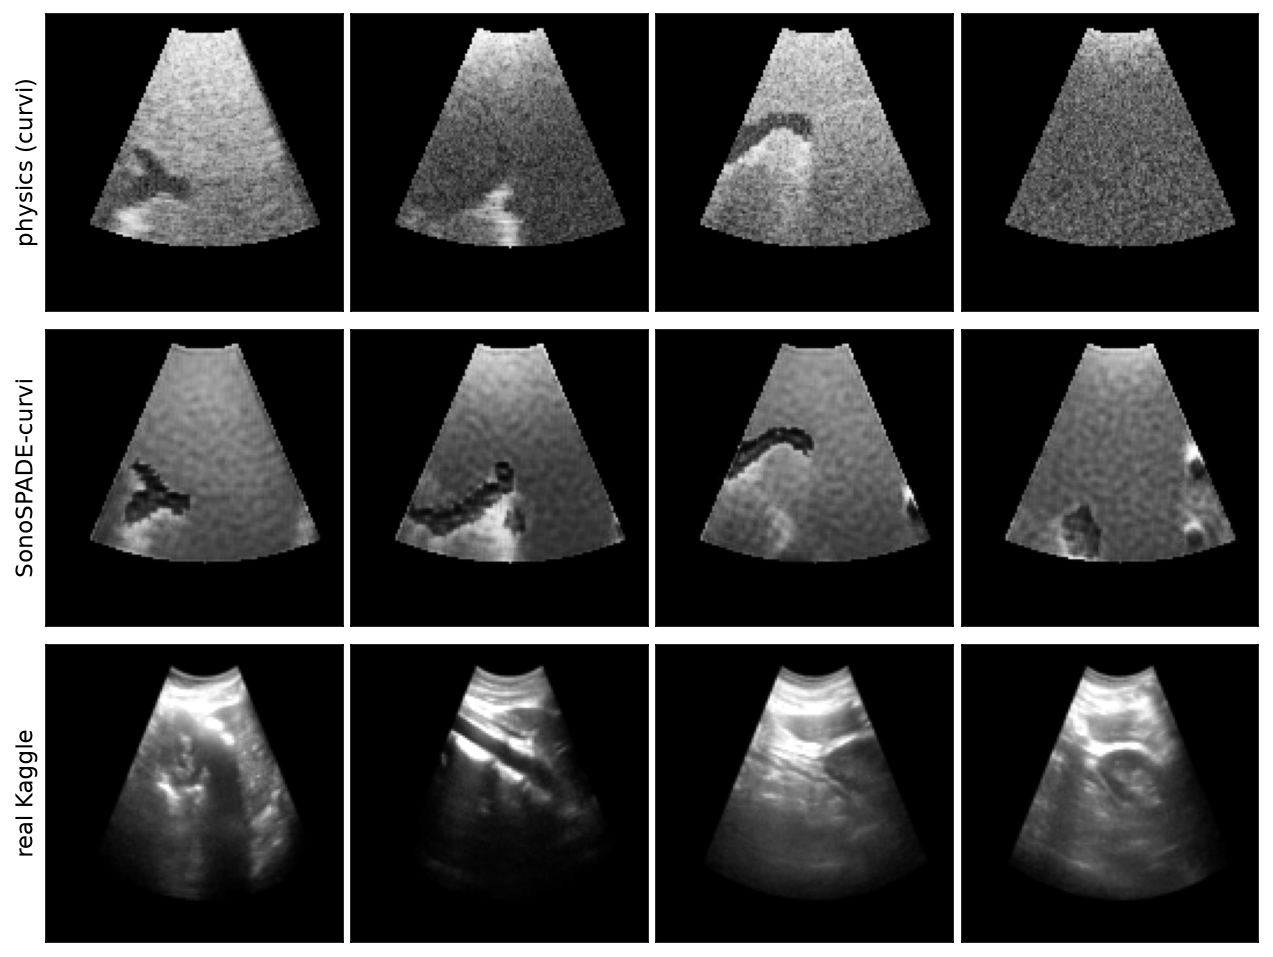
\includegraphics[width=0.48\linewidth]{figures/curvilinear.png}
\caption{Curvilinear remap (Experiment~A, Sec.~\ref{sec:tstr}). After warping into the measured sector
geometry, the curvilinear physics render (top), SonoSPADE-curvi (middle), and a real Kaggle frame (bottom)
share the same sector field. This is the geometry match that lifts downstream transfer in
Table~\ref{tab:tstr}.}
\label{fig:curvi}
\end{figure}

\subsection{Inference latency: real time, no GPU}
\label{sec:latency}
Because the stage runs inside a reinforcement-learning acquisition loop, per-frame latency, not peak realism, is the limiting factor. A single generator pass takes $66$\,ms on CPU ($15$ frames/s) and $12$\,ms on an integrated GPU ($85$ frames/s) at batch one, with \emph{no discrete GPU}(\texttt{scripts/bench\_latency.py}). 
A diffusion synthesizer instead runs $T$ denoising passes per frame: a representative ADM/SDM-style denoising U-Net (the family Echo-from-noise~\cite{stojanovski2023echofromnoise} builds on; $62$M parameters, sized to lower-bound the cost) costs $186$\,ms per pass on CPU, only about $2.7\times$ a SonoSPADE pass, but its $T$ passes make it two orders of magnitude slower \emph{per frame} at $T{=}50$ ($133\times$ on CPU) and up to three at full DDPM. 
For millions of frames, seconds per frame is too expensive. We give up whole-frame FID/KID for this real-time, GPU-free inference, and unlike the equally fast label-free baselines, SonoSPADE is per-tissue. 
We verified this in place inside a MuJoCo closed-loop acquisition environment, where the texture stage is not the bottleneck. Whether it also improves \emph{acquisition quality} is the subject of Sec.~\ref{sec:organrl}.

\subsection{Per-tissue texture improves an in-the-loop acquisition agent}
\label{sec:organrl}
The latency result shows the texture stage \emph{can} run in the loop; it does not show per-tissue texture
\emph{helps} the agent. That needs a task whose reward depends on per-tissue correctness, scored by a judge
\emph{fixed across} texture stages, not matched to each (the flaw that made our earlier goal-reaching
benchmark uninformative, Sec.~\ref{sec:limitations}). We build one: \emph{organ-conditioned acquisition}. 
A probe starts with the target organ partly in view and moves to bring it in; the per-step reward is the confidence of a frozen organ recognizer $J$ that the organ is present. $J$ is trained \emph{only on real} Kaggle frames and masks (never on synthetic output, so the reward is non-circular) and is the \emph{same} $J$ for every texture stage. The main metric is texture-independent: the ground-truth fraction of the acquired view that is the target organ.

Is the reward usable? On held-out simulator content, $J$'s liver IoU is \recSono{} for SonoSPADE versus \recCut{} (CUT) and \recCyc{} (CycleGAN), approaching the real-data ceiling \recCeil{} (Table~\ref{tab:organrl}, \rlSeeds{} seeds); the untranslated render scores \recPhys{}, \emph{above} both recolors, so part of the effect is structure preservation, not per-tissue texture alone. 
A fair comparison also trains all three translators on the \emph{same} real pool; an off-pool CUT checkpoint wrongly reverses the result. 
Trained under this reward (imitation-warm-started REINFORCE, \rlSeeds{} seeds, held-out patients), SonoSPADE reaches the highest ground-truth liver visibility, $\rlSono\,{\pm}\,\rlSonoSd$, above CUT (\rlCut{}), CycleGAN (\rlCyc{}), and the render (\rlPhys{}) from a static start of \rlStart{}, with all three per-seed differences positive and sign-consistent (directional, not significance-tested). 
Its reward signal is about twice as strong (\rewSono{} versus \rewCut{}--\rewPhys{}); the ground-truth margin is \emph{small} because the warm-start and liver's dominance already nearly solve the task. 
To our knowledge, this is the first evidence that per-tissue texture helps an in-the-loop agent under a fixed, real-trained
judge.

The effect is confined to liver: for kidney, spleen, and gallbladder \emph{no} translator (SonoSPADE included) yields a rendering the recognizer identifies (IoU ${\approx}\,0$), though the same $J$ scores them $0.3$--$0.8$ on \emph{real} data. 
The bottleneck is the simulator and translator failing to reproduce their appearance, not the recognizer, so the multi-organ claim rests on the offline metrics and the in-the-loop gain is shown for the organ that transfers.

\begin{table}[t]
\centering
\caption{Organ-conditioned liver acquisition (\rlSeeds{} seeds, held-out patients). Top: a fixed
real-trained recognizer $J$ recognizes SonoSPADE's liver far better than a recolor's (real-data ceiling
\recCeil{}). Middle: trained under $J$ as reward, SonoSPADE reaches the highest \emph{ground-truth} liver
visibility (static start \rlStart{}), higher in \rlSeeds{}/\rlSeeds{} seeds. Bottom: its reward signal is
${\sim}2\times$ stronger.}
\label{tab:organrl}
\begin{tabular}{lcccc}
\toprule
 & physics & CUT & CycleGAN & SonoSPADE\\
\midrule
$J$ liver recognition, IoU $\uparrow$        & \recPhys{} & \recCut{} & \recCyc{} & \textbf{\recSono{}}\\
Ground-truth liver acquired $\uparrow$       & \rlPhys{}  & \rlCut{}  & \rlCyc{}  & \textbf{\rlSono{}}\\
Reward signal ($J$ conf., secondary) $\uparrow$ & \rewPhys{} & \rewCut{} & \rewCyc{} & \textbf{\rewSono{}}\\
\bottomrule
\end{tabular}
\end{table}

\section{Limitations}
\label{sec:limitations}
Unpaired training matches per-tissue statistics, not exact speckle, so the output is training texture, not diagnostic imagery, and per-tissue fidelity is strong only for tissues acoustically distinct in B-mode. 
We validate on a \emph{single} dataset and anatomy (abdominal Kaggle, $60$ annotated real frames, $8$ CT cases); other anatomies and scanners are untested, and downstream Dice stays low even after the fixes, so transfer is directional, not clinical-grade. Our in-the-loop evidence is also bounded: it does not come from the earlier goal-reaching benchmark, whose per-texture \emph{matched} judge is not comparable across texture stages (a random policy scores ${\approx}0.36$ under one judge, ${\approx}0.03$ under another), and the organ-conditioned gain that replaces it is small, seed-consistent rather than significance-tested (\rlSeeds{} seeds), and liver-only.

\section{Conclusion}
SonoSPADE is a real-time, GPU-free, per-tissue ultrasound texture stage for closed-loop acquisition: conditioning on both a physics render and the tissue label slice makes texture per-tissue and controllable, supervised for free by a frozen simulator-pretrained segmenter with no real labels. 
After matching the sector geometry it overtakes the untranslated render on downstream transfer, and its per-tissue reward gives an in-the-loop agent the highest ground-truth liver visibility under a fixed real-trained judge. 
More broadly, a fast, controllable texture stage makes closed-loop acquisition simulation practical, a step toward training autonomous and robotic ultrasound acquisition in simulation.
The recipe trains on an ordinary laptop, and we hope it opens a research window to jointly improve realism, controllability, and speed.

\bibliographystyle{splncs04}
\bibliography{references}

\end{document}
